\documentclass{beamer}
\usefonttheme{serif}
\usetheme{boadilla}

\usepackage{amsthm, amsfonts, amsmath, amssymb} % Pacote para a definicao dos ambientes matematicos
\usepackage[brazilian]{babel}
\usepackage[utf8]{inputenc}
\usepackage[mathscr]{eucal}
\usepackage{tikz}
\usepackage{subcaption}
\usepackage{graphicx}
\usepackage{hyperref}
\usetikzlibrary{quotes, angles, intersections}
\newcommand{\R}{\mathbb{R}}
\newcommand{\D}{\mathscr{D}}
\newcommand{\Pp}{\mathscr{P}}
\newcommand{\bigO}{\mathscr{O}}
\newcommand{\Cc}{\mathscr{C}}
\newcommand{\E}{\mathscr{E}}
\newcommand{\F}{\mathscr{F}}
\newcommand{\Ww}{\mathscr{W}}
\newcommand{\Rr}{\mathscr{R}}
\newcommand{\norm}[2][2]{\left\lVert#2\right\rVert_{#1}}
\newcommand{\sigla}[2]{#2 (#1)}
\newcommand{\citeonline}[1]{\cite{#1}}

\newtheorem{thm}{Theorem}
\newtheorem{prp}{Proposition}
\newtheorem{lem}{Lemma}
\theoremstyle{definition}
%\newtheorem{definition}{Definition}[section]

\author{Danilo Tedeschi}
\title{New Exact Algorithms for Planar Maximum Covering Location by Ellipses Problems}
\institute{Universidade de São Paulo}
\date{25 de Outubro de 2019}


\begin{document}
	
	\begin{frame}[t,plain]
		\titlepage
		
		\footnotesize This research has been funded by Cordenação de Aperfeiçoamento de Pessoal de Nível Superior (CAPES).
	\end{frame}

	\begin{frame}{Introduction}{Related problems}

		\sigla{MCLP}{The Maximum Covering Location Problem} 
		\begin{itemize}
			\item Introduced in \cite{church:1974},
			\item Maximize the coverage demand vertices on a graph,
			\item Choose the location (vertex) of a fixed number of facilities,
			\item A demand vertex is considered covered if a facility is located within its coverage radius.
		\end{itemize}
	\end{frame}

	\begin{frame}{Introduction}{Related problems}
	
	\sigla{PMCLP}{The Planar Maximum Covering Location Problem} 
	\begin{itemize}
		\item Introduced in \cite{church:1984},
		\item Maximize the coverage demand vertices in $\R^2$,
		\item Choose the location (could be anywhere in $\R^2$) of a fixed number of facilities,
		\item A demand vertex is considered covered if a facility is located within its coverage radius,
		\item Several distance functions were studied. We are particularly interested in the Euclidean PMCLP.
	\end{itemize}
	\end{frame}

\begin{frame}{Introduction}
	
	We propose algorithms for two versions of PMCLP.
	
\end{frame}

\begin{frame}{Introduction}{MCE}
	Planar Maximum Covering Location by Ellipses Problem (MCE):
	\begin{itemize}
		\item Introduced in \cite{canbolat}, 
		\item Mixed Non-linear optimization and a heuristic method in \cite{canbolat},
		\item Exact method, solving convex sub-problems in \cite{andreta}.
	\end{itemize}

	\begin{block}{Our algorithm}		
		Based on the approach used for the Euclidean PMCLP in \cite{church:1984}.
		Transform MCE into a combinatorial optimization problem.
	\end{block}
\end{frame}

\begin{frame}{Introduction}{MCER}
	Planar Maximum Covering Location by Ellipses with Rotation Problem (MCER):
	\begin{itemize}
		\item Introduced in \cite{andreta}, 
		\item Exact method, solving many optimization sub-problems in \cite{canbolat},
		\item Heuristic method in \cite{andreta}.
		\item Much more challenging than MCE.
	\end{itemize}
	
	\begin{block}{Our algorithm}		
		Transforms MCER into a combinatorial optimization problem.
	\end{block}
\end{frame}

\begin{frame}{Introduction}{Ellipse}
	The shape of an ellipse is given by its major-axis and minor-axis, $(a, b) \in \mathbb{R}^2_{>0}$, $a > b$.
	
	\begin{figure}[H]
		\centering
		
		%\caption{The ellipse as a parametric curve.}
		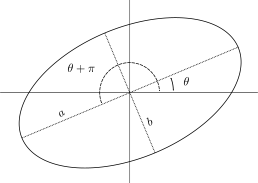
\includegraphics[scale=.3]{../tex/figures/rotated_ellipse.pdf}
		\label{fig:ellipse_params}
		\caption{An ellipse with shape parameters $a$ and $b$.}
	\end{figure}
	
\end{frame}

\begin{frame}{Introduction}{Ellipse}
	An ellipse can be defined using a norm function $||\cdot||_{a,b,\theta}$ given by
	\begin{equation*}
		||x||_{a,b, \theta}=\left|\left|
		\left(\begin{array}{rr}
		\cos{\theta} & \sin{\theta}\\
		\sin{\theta} & -\cos{\theta}
		\end{array}
		\right)
		\left(\begin{array}{cc}
		1/a & 0\\
		0 & 1/b
		\end{array}\right) x \right|\right|_2.
	\end{equation*}
\end{frame}

\begin{frame}{Problem definition}
	%\begin{block}{Definition}
	An instance of both MCE and MCER is given by
	\begin{itemize}
		\item A demand set $\Pp:=\{p_1, \dots, p_n\}$, $p_j \in \R^2$;
		\item Each point has a weight $\Ww := \{w_1, \dots, w_n\}$, $w_j \in \R_{\ge0}$;
		\item A list of shape parameters $\Rr := \{(a_1, b_1); \dots; (a_m, b_m)\}$, $(a_j, b_j) \in \R^2_{>0}$, with $a_j > b_j$.
	\end{itemize}
\end{frame}

\begin{frame}{Problem definition}
	\begin{figure}
		\begin{subfigure}{.4\textwidth}
			\centering
			\includegraphics[scale=.55]{../article/figures/MCE_TA04}
			\caption{}
			\label{fig:MCE_TA04}
		\end{subfigure}
		\begin{subfigure}{.4\textwidth}
			\centering
			\includegraphics[scale=.55]{../article/figures/MCER_TA04}
			\caption{}
			\label{fig:MCER_TA04}
		\end{subfigure}
		\caption{Solutions for the same instance of (a) MCE, and (b) MCER.}
		\label{fig:TA04}
	\end{figure}
\end{frame}

\begin{frame}{Problem definition}{More notation}
	
	\begin{block}{Weight function}
	Let $w\colon 2^\Pp \to \R$ be a function defined as
	
	\begin{equation*}
	w(A) = \sum_{j \colon p_j \in A} w_j.
	\end{equation*}
	
%	which takes a subset of $\Pp$ and returns the sum of the weights of the points in that subset.
	\end{block}

\begin{block}{MCE's solution}
	$Q:=(q_1, \dots, q_m) \in \R^{2m}$.
\end{block}

\begin{block}{MCER's solution}
	%$Q:=(q_1, \dots, q_m)$.\\
	$Q:=((q_1, \theta_1); \dots; (q_m, \theta_m)) \in (\R^2\times [0, \pi))^m$.
\end{block}
	
	%(Only used to make the text more clear)
\end{frame}

\begin{frame}{Problem definition}{MCE}
	Let $E_j \colon \R^2 \to \R^2$ be the coverage region of the $j$-th ellipse defined as
	\begin{equation*}
	E_j(q) = \{x \in \R^2\colon ||x-q||_{a,b,0} \le 1\}.
	\end{equation*}
	Then, MCE is defined as the optimization problem:
	\begin{equation*}
	\max_{Q}  w\left(\bigcup_{j=1}^m\Pp \cap E_j(q_j)\right).
	\end{equation*}
\end{frame}

\begin{frame}{Problem definition}{MCER}
	Let $E_j \colon \R^2\times[0, \pi) \to \R^2$ be the coverage region of the $j$-th ellipse defined as
	\begin{equation*}
	E_j(q,\theta) = \{x \in \R^2\colon ||x-q||_{a,b,\theta} \le 1\}.
	\end{equation*}
	Then, MCER is defined as the optimization problem:
	\begin{equation*}
	\max_{Q}  w\left(\bigcup_{j=1}^m\Pp \cap E_j(q_j,\theta_j)\right).
	\end{equation*}
	
	\begin{block}{Remark}
		For the one-facility MCE and MCER, we omit the index referring to the ellipse.
	\end{block}
\end{frame}

\begin{frame}{MCE}
	$\{p_1, p_2, p_3\} \subset E(q)$
	\begin{figure}
		\centering
		\includegraphics[scale=.55]{figures/mce-mwc0}
		\caption{A solution for the one-facility MCE.}
	\end{figure}
\end{frame}

\begin{frame}{MCE}
	$\{p_1, p_2, p_3\} \subset E(q) \implies q \in E(p_1) \cap E(p_2) \cap E(p_3)$.
	\begin{figure}
		\centering
		\includegraphics[scale=.55]{figures/mce-mwc}
		\caption{A solution for the one-facility MCE.}
	\end{figure}
\end{frame}

\begin{frame}{MCE}
	In general we have
	\begin{equation*}
	A = \Pp \cap E(q) \implies 	q \in \cap_{p \in A} E(p),
	\end{equation*}
and
	\begin{equation*}
	q' \in \cap_{p \in A} E(p) \implies	A \subset E(q').
	\end{equation*}
	
	\begin{block}{Intersection region of ellipses}
		By \cite{bi}, we have that if $|A|>1$, there is at least one intersection between two ellipses in the border of $\cap_{p\in A} E(p)$.
	\end{block}
\end{frame}

\begin{frame}{MCE}
	$\{q_1, q_2, q_3\} \subset \bigcup_{1 \le i < j \le 3} \partial E(p_i) \cap \partial E(p_j)$.
	\begin{figure}
		\centering
		\includegraphics[scale=.55]{figures/mce-mwc1}
		\caption{A solution for the one-facility MCE.}
	\end{figure}
\end{frame}

\begin{frame}{MCE}
	In general, we have
	\begin{equation*}
	|\partial E(u) \cap \partial E(v)| \le 2, 
	\end{equation*}
	and that $\partial E(u) \cap \partial E(v)$ can be determined analytically.
\end{frame}

\begin{frame}{MCE}{Candidate List Set}
	
	Based on \cite{church:1984}, we define a Candidate List Set (CLS) for each facility as follows.
	
	\begin{definition}\label{def:cls_mce}
		Given an instance of MCE, for all $k \in \{1, \dots, m\}$, we define the CLS for the $k$-th ellipse as
		\begin{equation*}
		S_k = \Pp \cup \left(\bigcup_{1 \le i < j \le n} \partial E_k(p_i) \cap \partial E_k(p_j) \right).
		\end{equation*}
	\end{definition}
\end{frame}

\begin{frame}{MCE}{Main result}
	\begin{thm}\label{thm:mce}
		Given an instance of MCE, and $S_1, \dots, S_m$ as defined previously, then the set $$\Omega = \{(q_1, \dots, q_m) \colon \textnormal{ for all }q_k \in S_k \}$$ contains an optimal solution of MCE and $|\Omega| \le n^{2m}$. 
	\end{thm}

\begin{itemize}
	\item Notice that $|S_k| \le n(n+1)/2 \le n^2$.
	\item An algorithm with $\bigO(mn^{2m+1})$ runtime complexity can be implemented.
\end{itemize}

\end{frame}


%%% E3P

\begin{frame}{Determining Every Center and Angle of Rotation of An Ellipse Given Its Shape and Three Points that It Must Contain}
	Given
	\begin{itemize}
		\item The coverage region function of an ellipse $E \colon \R^2 \times [0, \pi) \to \R^2$.
		\item Three points $u, v, w \in \R^2$.
	\end{itemize}
Let us call E3P the problem whose solution is given by $(q, \theta) \in \R^2 \times [0, \pi)$, such that

$$\{u, v, w\} \subset \partial E(q, \theta).$$

We want to compute every solution of E3P.

We did not find any work on E3P in the literature.
\end{frame}

\begin{frame}{E3P}
	\begin{figure}
		\centering
		\includegraphics[scale=.4]{../tex/figures/e3p_4sols}
		\caption{Example of every solution for an instance of E3P.}
	\end{figure}
\end{frame}

\begin{frame}{E3P}{Transforming the problem}
	Let us define a function $\varphi \colon \R^2 \times [0, \pi) \to \R^2$ that transforms the problem as follows.
	\begin{figure}
		\centering
		\includegraphics[scale=.7]{../article/figures/circumscribed-circle}
		\caption{Transforming a solution of E3P into a solution of the circumcircle problem.}
	\end{figure}
\end{frame}

\begin{frame}{E3P}{Transforming the problem}
	If $u$ is at the origin, this function can be described as
	\begin{equation*}%\label{eq:trpnts}
	\varphi(p, \theta)=\left[\begin{array}{cc}
	\frac{b}{a}&0\\
	0&1
	\end{array}\right]
	\left[\begin{array}{cc}
	\cos{\theta}&\sin{\theta}\\
	-\sin{\theta}&\cos{\theta}
	\end{array}\right]\left[\begin{array}{c}
	p_x\\
	p_y
	\end{array}\right].
	\end{equation*}
	
	\begin{itemize}
		\item For a fixed angle, $\varphi$ is bijective, we refer to $\varphi^{-1}$ as its inverse.
		\item Let us denote by $\Lambda(\theta)$ as the triangle with vertices $\varphi(u), \varphi(v), \varphi(w)$.
		%\item if $\theta$ The circumscribed circle of $\Lambda(\theta)$ has radius $b$.
		\item E3P is equivalent to determining $\theta$, such that the circumscribed circle of $\Lambda(\theta)$ has radius $b$.
	\end{itemize}	
\end{frame}

\begin{frame}{E3P}{Transforming the problem}
	A circle is uniquely defined by $\Lambda(\theta)$, and its radius and center can be determined analytically \cite{weisstein}. 
	
	Let $|\Lambda(\theta)|$ be the area of $\Lambda(\theta)$, and imposing that the radius of that circle is equal to $b$, we define a function $\xi \colon [0, \pi) \to \R$ whose roots determine solutions of E3P. 
	
	\begin{equation*}\label{eq:xi}
	\xi(\theta) = 16b^2|\Lambda(\theta)|^2 - \norm{\varphi(v, \theta)}^2\norm{\varphi(w, \theta)}^2\norm{\varphi(v, \theta)-\varphi(w, \theta)}^2.
	\end{equation*}
\end{frame}

\begin{frame}{E3P}
	\begin{lem}\label{lema:e3p}
		E3P has at most six solutions.
	\end{lem}
\begin{itemize}
	\item $\xi$ can be written as $\sum_{0 \le j+k \le 6} c_{j,k} \cos^j\theta \sin^k\theta$,
	\item It is a real trigonometric polynomial, 
	\item By \cite[p.~150]{powell}, it has at most $12$ roots in $[0, 2\pi)$,
	\item As ellipses are symmetrical, we can dismiss half of the roots.
\end{itemize}
\end{frame}

\begin{frame}[allowframebreaks]
	\frametitle{References}
	\bibliographystyle{acm}
	\bibliography{../references}
\end{frame}
	
\end{document}